\documentclass[
	12pt,
	a4paper,
	BCOR10mm,
	%chapterprefix,
	DIV14,
	listof=totoc,
	bibliography=totoc,
	headsepline
]{scrreprt}

\usepackage[T1]{fontenc}
\usepackage[utf8]{inputenc}
%\usepackage{ngerman}

\usepackage{lmodern}
\usepackage[german]{babel}

\usepackage[footnote]{acronym}
\usepackage[page,toc]{appendix}
\usepackage{fancyhdr}
\usepackage{float}
\usepackage{graphicx}
\usepackage[pdfborder={0 0 0}]{hyperref}
\usepackage[htt]{hyphenat}
\usepackage{listings}
\usepackage{lscape}
\usepackage{microtype}
\usepackage{nicefrac}
\usepackage{subfig}
\usepackage{textcomp}
\usepackage[subfigure,titles]{tocloft}
\usepackage{units}
\usepackage{amssymb}
\usepackage{pgfplots}

\lstset{
	basicstyle=\ttfamily,
	frame=single,
	numbers=left,
	language=C,
	breaklines=true,
	breakatwhitespace=true,
	postbreak=\hbox{$\hookrightarrow$ },
	showstringspaces=false,
	tabsize=4
}

\renewcommand*{\lstlistlistingname}{Listingverzeichnis}

\renewcommand*{\appendixname}{Anhang}
\renewcommand*{\appendixtocname}{Anhänge}
\renewcommand*{\appendixpagename}{Anhänge}

\begin{document}

\begin{titlepage}
	\begin{center}
		{\titlefont\huge Vorhersage von E/A-Leistung im Hochleistungsrechnen unter der Verwendung von neuronalen Netzen\par}

		\bigskip
		\bigskip

		{\titlefont\Large --- Bachelorarbeit ---\par}

		\bigskip
		\bigskip

		{\large Arbeitsbereich Wissenschaftliches Rechnen\\
		Fachbereich Informatik\\
		Fakultät für Mathematik, Informatik und Naturwissenschaften\\
		Universität Hamburg\par}
	\end{center}

	\vfill

	{\large \begin{tabular}{ll}
		Vorgelegt von: & Jan Fabian Schmid \\
		E-Mail-Adresse: & \href{mailto:2schmid@informatik.uni-hamburg.de}{2schmid@informatik.uni-hamburg.de} \\
		Matrikelnummer: & 6440383 \\
		Studiengang: & Computing in Science - SP. Physik \\
		\\
		Erstgutachter: & Dr. Julian Kunkel \\
		Zweitgutachter: & Prof. Dr. Thomas Ludwig\\ \\
		Betreuer: & Dr. Julian Kunkel \\
		\\
		Hamburg, den 17.12.2015
	\end{tabular}\par}
\end{titlepage}

\chapter*{Abstract}

\thispagestyle{empty}



\tableofcontents

\chapter{Einleitung}
\label{Einleitung}

\textit{%
Im folgenden wird zunächst kurz dargelegt mit welcher Problemstellung sich diese Thesis befasst, welches Ziel verfolgt wird, und wie dieser Text im Weiteren aufgebaut sein wird.
}
\bigskip

\section{Motivation}

Hochleistungsrechnen ist in der Wissenschaft ein Thema mit zunehmender Signifikanz, viele komplexere Fragestellungen, insbesondere in den Naturwissenschaften und der Informatik, können z.B. nur in einer effizienten Weise durch Analyse einer Simulation eines Modells gelöst werden. Der extensive Rechenaufwand solcher Simulationen erfordert, dass Wissenschaftler nicht am eigenen Computer rechnen, sondern hierfür die Dienste eines Hochleistungszentrum in Anspruch nehmen. 
Die Entwicklung der Computer-Hardware in den vergangen Jahrzehnten drängte die Hochleistungszentren dazu für den gewünschten Leistungsgewinn in stark parallelisierte Systeme zu investieren. Sodass, statt einzelner sehr schneller Prozessoren heutzutage viele Tausend Prozessoren vernetzt arbeiten. Diese horizontale Leistungssteigerung am Hochleistungsrechner umgeht die technischen Flaschenhälse, welche die Leistung eines einzelnen Prozessors beschränkt, die zur Verfügung stehende Leistung wird dadurch allerdings schwieriger nutzbar. 
Einerseits liegt dies am großen  technische Aufwand, der zur Vernetzung der Recheneinheiten notwendig ist, andererseits liegt es an der komplexen Programmierung der Software, welche die Parallelität des Rechners berücksichtigt. Insbesondere ist es auch bei der Ein-/Ausgabe (E/A) von erforderlichen Dateien und Ergebnissen des Programms wichtig, dass sie parallel durchgeführt wird.
Um die Wissenschaftler beim Programmieren zu unterstützen, gibt es hilfreiche Tools zur Fehlerdiagnostik, Leistungsanalyse, Visualisierung des Programms und der Ergebnisse, sowie zum Parallelisieren von Programmcode. Wünschenswert ist es dabei, wenn diese Tools die Optimierungen möglichst selbstständig durchführen können, sodass der Wissenschaftler sich auf die Funktionalität seines Programms konzentrieren kann, statt sich mit Leistungsoptimierung abzulenken.

\section{Problemstellung}

Im Bereich der Leistungsanalyse stellt sich unter anderem die Problematik der effizienten Ausnutzung der verschiedenen Puffer-Speicher (Caches), wie Arbeitsspeicher, und die direkt auf dem Prozessor liegenden Caches. Autonome Tools zur Optimierung der E/A können versuchen die Dauer von Dateizugriffen vorherzusagen \textbf{(warum?)}. Diese Arbeit versucht dies mit dem Hilfsmittel neuronaler Netze zu erreichen. 

\section{Ziele der Thesis}
Main goal:\\
A neural network that is reliable in predicting performance of HPC-IO with sufficient quality\\

Subgoals:\\
Knowing which data can be provided by SIOX\\
Identify interesting (data mining) features, that can be derived from the available data\\
Having an understanding of what kind of neural network is suitable for the task\\
A measure for adequate quality of an IO-performance predictor \\
Benchmark of different predictors using different approaches\\
Implementation of a predictor module for SIOX for online evaluation of application performances\\

\section{Strukturierung}
Nachdem in diesem Kapitel die Metaebene der Thesis behandelt wird, soll das zweite Kapitel alle nötigen Hintergrundinformationen zum Verstehen der Thematik und der hier angewandten Ansätze liefern. Das dritte Kapitel beschäftigt sich mit bereits vorhandenen Ansätzen und Arbeiten zur Problemstellung. Im vierten Kapitel werden die Konzepte, sowie die Implementierung, der verschiedenen Modelle beschrieben, die als potenzielle Lösungen des Problems entwickelt und getestet wurden. Die Evaluierung der verschiedenen Lösungsansätze wird daraufhin im fünften Kapitel vorgenommen. Im sechsten Kapitel wird untersucht, welche Lösungsansätze für welche Anwendungsfälle am besten geeignet sind, um dann mit diesen Erkenntnissen im siebten Kapitel ein Fazit der Arbeit zu ziehen.

\chapter{Hintergrund}

\section{Ein-/Ausgabe}
\label{E/A}
Wie werden Dateien abgelegt, wie greift man darauf zu.
Wie funktioniert Caching? Read ahead, Write ahead? \textbf{Was soll hier so hin?}
\medskip

Als Ein-/Ausgabe (E/A) bezeichnet man jedweden Austausch von Informationen eines Informationssystems mit der Außenwelt (Wiki). Durch Eingaben erhält der Rechner auszuführende Befehle, die Programme und Funktionen mit denen er etwas ausführen soll, sowie die Daten, die verarbeitet werden sollen. Eine Ausgabe des Rechners gibt dem Nutzer Informationen zum inneren Zustand des Systems und er erhält die Ergebnisse seiner Eingaben.
Im Kontext dieser Arbeit handelt es sich bei Ein-/Ausgaben um Dateien, die vom Computersystem von einem Datenträger eingelesen und wieder darauf geschrieben werden.
Die in den Testsystemen verwendeten Datenträger sind Festplattenlaufwerke, bei diesen werden Informationen durch magnetische Polarisierung von Speicherzellen auf Magnetscheiben gespeichert und durch Abtastung dieser Magnetisierung mit einem Lesekopf ausgelesen. (\textbf{Bild einer Festplatte})
Festplatten sind in Datenblöcke (auch Sektoren) unterteilt, diese bilden die kleinste Einheit, die von dem Medium gelesen bzw. darauf geschrieben werden kann. Durch eine eindeutige Adressierung dieser Sektoren kann der Schreib-/Lesekopf durch Aus- und Einfahren, sowie einer Drehung der Magnetscheibe, direkt auf den gewünschten Datenblock zugreifen.
Aufgrund des vergleichsweise geringen Durchsatzes, und insbesondere wegen der großen Latenz bei der Durchführung von Festplattenaufrufen, sind zwischen Festplatte und den tatsächlichen Recheneinheiten im Prozessor mehrere Schichten von Speichern zwischengeschaltet. Von der Festplatte gelesene Daten befinden sich zunächst auf dem Arbeitsspeicher und werden dann in die auf dem Prozessor liegenden Pufferspeicher (Caches) geladen. In den verschiedenen Cache-Ebenen geschieht vergleichbares, die Ebenen gehen von kleinen, sehr schnellen zu größeren, langsameren Speichern über, üblich sind hier zwei oder drei Level. 
Die Zugriffszeit auf eine Datei ist durch diese Struktur stark davon abhängig in welcher Speicherebene es einen Treffer zu den gesuchten Speicheradressen gibt. Wenn die Datei bereits vollständig im Level 1 Cache liegt, ist sie schon nach wenigen Prozessorzyklen geladen, wenn sie aus dem Arbeitsspeicher geholt werden muss, braucht es mehrere hundert Prozessorzyklen. Das lesen von der Festplatte dauert hingegen einige Millionen Zyklen (\textbf{Link? duartes.org}). Im wesentlichen kann also unterschieden werden, ob eine Datei "gecached", sich also im Arbeitsspeicher oder Prozessor-Cache befindet, oder noch von der Fesplatte geladen werden muss.
Verschiedene Caching-Strategien erlauben eine noch effizientere Nutzung der Zwischenspeicher. Ein Beispiel ist das Einschalten der Read-Ahead-Einstellung, dadurch werden weitere Sektoren im Cache zwischengespeichert, die sich in der unmittelbaren physischen Umgebung auf dem  Speichermedium befinden. Falls ein Programm fortlaufend über einen großen Datenbereich arbeitet, weil dort beispielsweise direkt hintereinander Bilddateien eines Fotoalbums befinden, das gerade im Präsentationsmodus gezeigt wird, so ist der Zugriff auf ein weiteres Bild für das E/A-System nicht mehr 'überraschend'. Statt erst in dem Moment des E/A-Aufrufs des nächsten Bildes die erforderlichen Datenblöcke von der Festplatte zu lesen, befinden sich diese nun bereits in einem der vorgeschalteten Zwischenspeicher. Diese Caching-Strategie macht offensichtlich nur Sinn, wenn ein solches sequentielles Zugriffsverhalten eines Programms stattfindet. Wenn aufeinanderfolgende Zugriffe in unterschiedlichen Bereichen der Festplatte Datenblöcke anfordern, würde bei dieser Strategie immerzu zusätzlicher Aufwand für das lesen der umgebenden Daten betrieben, ohne davon einen Nutzen zu haben. 
Eine weitere Caching-Strategie ist das Write-Back. Beim Write-Through werden Schreibbefehle, die zunächst nur direkt im Cache umgesetzt werden, direkt in den Arbeitsspeicher übernommen. Cache und Arbeitsspeciher sind so immer in einem gültigen Zustand --- 

\section{Hochleistungsrechnen}
Wofür HPC? c
Was zeichnet HPC aus? c
Ein-/Ausgabe im HPC  c
Besondere herausforderungen
\medskip

Man spricht von Hochleistungsrechnen, wenn der Rechenaufwand eines Programms außerhalb dessen liegt, was ein einzelner Desktop-Computer in vertretbarer Zeit bearbeiten kann.
Die im Hochleistungsrechnen verwendeten Computer werden als Superrechner bezeichnet (wiki Superrechner), hierbei handelt es sich heutzutage üblicherweise um Rechnerverbünde (englisch: Cluster) in denen große Anzahlen Prozessoren und Speichermedien zusammengeschaltet werden.
Notwendig wird Hochleistungsrechnen in der Forschung für die Simulation von numerischen Modellen aus verschiedensten Bereichen, beispielsweise zur Mehrkörpersimulation in der Astronomie, für Strömungssimulationen oder zur Berechnung von Klimaprognosen.
Wichtige Themen im Hochleistungsrechnen sind die Ausnutzung der zur Verfügung stehenden Leistung, das Erkennen und Beheben von Fehlern des genutzten Programmcodes, die Bereitstellung der Rechen- und Speicherkapazitäten, sowie die Energieeffizienz von Hard- und Software.
Um den Superrechner gut ausnutzen zu können ist eine effiziente Ein-/Ausgabe bei vielen Anwendungen von großer Wichtigkeit, da die Menge der anfallenden Datenmengen wesentlich stärker ansteigt, als die Geschwindigkeit der Verbindungen zwischen den verschiedenen Speichermedien und -orten. So steigt beispielsweise die Rechenleistung und die Speicherkapazität beim dem Superrechner des Deutschen Klimarechenzentrum (DKRZ) gegenüber dem Vorgänger wesentlich stärker an, als der mögliche Datendurchsatz (\textbf{Verweis}).
Die in \ref{E/A} beschriebene Ein-/Ausgabe erweitert sich im Rechnerverbund zur parallelen E/A, dies bedeutet einerseits, dass eine Datei von mehreren Prozessen zeitgleich gelesen und bearbeitet werden kann, und andererseits, dass eine Datei über mehrere Festplatten verteilt sein kann. Diese Parallelität hat einen wesentlichen Einfluss auf die Aufgabe der E/A-Leistungsvorhersage, denn statt nur den Aufwand der Arbeitsschritte auf einer einzelnen Festplatte abzuschätzen, müssen hier die verstrickten Zusammenhänge zwischen Netzwerken von Festplatten und Rechnern, den jeweiligen Auslastungen der Komponenten, sowie Priorisierungen bestimmter Aufgaben und Instanzen.\\
\textbf{Dies woanders hin?}
Die Erfassung dieser Informationen wäre sehr aufwendig, sodass dies zur Zeit nicht möglich ist. Die Genauigkeit einer Vorhersage von E/A-Leistung eines parallelen Systems sollte daher systematisch ungenauer sein, als die zu einem seriellen System.


\section{Ein-Ausgabe Optimierung mit SIOX}
Ziele
Vorgehen
Wofür diese Arbeit?

\cite{UMLTPTPONI15} The SIOX framework [13,14] aims to become a holistic approach covering the
full cycle of monitoring, analysis, machine learning of the adequate settings and
their automatic enactment.

\section{Maschinelles Lernen}
Wozu c
Verschiedene Klassen, un -/ supervised c
kmeans
regresson trees
neuronale netze -> verweis
Bagging

Maschinelles Lernen gehört in die Bereiche künstliche Intelligenz und automatisierte Wissensgenerierung. Verfahren dieser Disziplin versuchen durch intelligentes lernen von Mustern Vorhersagen und Entscheidungen, wie die Zuordnung zu einer bestimmten Klasse, zu treffen. Intelligent bedeutet hierbei (beispielweise), dass vorgegebene Informationen nicht schlicht auswendig gelernt und wiedergegeben werden, sondern von diesen Informationen abstrahiert wird, um Gesetzmäßigkeiten innerhalb der Trainingsdaten zu erkennen. Ein Verfahren oder Algorithmus des maschinellen Lernens erstellt ein Modell, welches Aussagen über die Datenmenge trifft, die zu Verfügung stand und eventuell Vorhersagen über Daten trifft, die ihm beim Lernen nicht bekannt waren. 
Zu unterscheiden sind Verfahren des überwachten und des unüberwachten Lernens. Während beim überwachten Lernen die idealen Ausgaben zu den Eingabedaten vorgegeben werden, wird beim unüberwachten Lernen kein bestimmtes Ergebnis erwartet, stattdessen muss der Algorithmus versuchen den Informationen inhärente Abhängigkeiten und Zusammenhänge zu erkennen.
Je nach Art der behandelten Daten sind die Modelle von Verfahren, die Vorhersagen über neue Daten treffen sollen, Klassifikationsmodelle oder Regressionsmodelle. Das Klassifikationsmodell ordnet Datenpunkte einer Klasse von Daten mit ähnlichen Eigenschaften zu, die verschiedenen Klassen müssen beim Erstellen des Modells bekannt sein und Beispiele als Datenpunkte dieser Klasse vorgegeben werden. Es wird also eine qualitative Aussage anhand dieser Einordnung in Gruppen über die einzelnen Datenpunkte getroffen. Dagegen wird beim Regressionsmodell eine quantitative Aussage über die Zusammenhänge zwischen den Attributen der Daten getroffen. Das Modell sagt einen bestimmten Wert für ein Attribut der Datenpunkte voraus.  
Die Trainingsdaten sind die Informationen, die dem Algorithmus bekannt sind, von diesen versucht er zu lernen. Falls ein Testdatensatz vorliegt, kann damit anschließend die berechnete Ausgabe zu bisher unbekannten Daten bewertet werden. Sowohl Trainingsdaten, sowie Testdaten enthalten gemessene Werte zu den Attributen, von denen gelernt werden soll (Eingabewerte). Ein Attribut ist eine messbare Größe des Systems, das untersucht wird. Dies könnte beispielsweise bei einem Datensatz über Blumen die Farbe der Blütenblätter sein. Ein Datenpunkt beschreibt eine Instanz des untersuchten Systems (z.B. ein exemplar der Blume), dazu enthält er einen gemessenen Wert zu jedem Attribut. Die Datenpunkte der Trainingsdaten beim überwachten Lernen, enthalen auch die "Lösungen" (die gesuchten Ausgabewerte) zu den Attributen, dessen Werte der Algorithmus vorhersagen soll. Diese Informationen werden dann beim Test vorenthalten, sodass durch den Vergleich zwischen tatsächlicher und vorhergesagter Lösung Rückschlüsse auf die Qualität der Vorhersagen gezogen werden können.
Zur Anwendung eines Verfahrens des maschinellen Lernens müssen zunächst Kriterien bzw. Leistungsmetriken eingeführt werden, anhand derer die Qualität der Vorhersagen und Entscheidungen gemessen werden können. Einerseits zum Vergleich verschiedener Ansätze, aber insbesondere für den Lernprozess des Algorithmus selbst, damit dieser sozusagen aus seinen Fehlern und Erfolgen lernen kann. Einfache Metriken wären beispielsweise für einen Klassifizierungsalgorithmus der Anteil falsch zugeordneter Datenpunkte.
Oft is es notwendig die zur Verfügung stehenden Daten aufzubereiten, bevor ein maschineller Lernalgorithmus effizient und korrekt Informationen aus diesen ableiten kann. So weist Alpaydin \cite{Alpaydin:2010:IML:1734076} (Seite 13-15) auf fehlerhafte Daten hin, die durch zufälligen Messfehler oder eine systematisch inkorrekte Messung entstanden sind. Zudem schreibt er, dass Teile der Daten überflüssig sein können, da sie redundant sind oder keine relevanten Informationen enthalten. Problematisch sind auch widersprüchliche (engl. inconsistent) Datenpunkte, hierbei stellen mehrere Datenpunkte dem maschinellen Entscheider die selben Eingabewerte zur Verfügung, sodass dieser sie nicht unterscheiden kann, sie haben jedoch unterschiedliche Ausgabewerte \cite{Alpaydin:2010:IML:1734076} (Seite 14). Mit all diesen Problemen muss, unter Beachtung der Eigenschaften des vorliegenden Datensatzes, bei der Aufbereiung der Daten sinnvoll umgegangen werden. So können Ausreißer bei den Daten aussortiert werden, da diese eventuell durch eine Fehlmessung entstanden sind. Widersprüchliche Datenpunkte können zusammengefasst werden, indem sie zusammen einen neuen Datenpunkt mit eindeutigen Ausgabewerten bilden (dies könnten die Mittelwerte sein). \\
Unüberwachtes Lernen findet bei der Clusteranalyse statt, Kantardzic beschreibt Clusteranalyse folgendermaßen: "Cluster analysis is the formal study of methods and algorithms for natural grouping, or clustering, of objects according to measured or perceived intrinsic characteristics or similarities." \cite{kantardzic2011data} (Seite 250). Ein einfaches und anschauliches Beispiel sind Punkte im zweidimesionnalen Raum, die hinsichtlich ihrer Position gruppiert werden. ( \textbf{BILDER SELBER MACHEN HIERZU} )
Ein einfacher Clustering-Algorithmus ist der k-Means-Algorithmus. Bei diesem muss zunächst die Anzahl Cluster $k$ festgelegt werden. Die $k$ Mittelwerte der Cluster mit zufälligen Werten initialisiert. Dann wird jeder Datenpunkt dem Cluster zugeordnet, dessen Mittelwert seinem am dichtesten ist. Danach werden die Mittelwerte der Cluster anhand der Ihnen zugeordneten Punkte mit einer beliebigen Metrik berechnet und gesetzt. Das Neuzuordnen der Punkte und Berechnen der Mittelwerte wird nun solange wiederholt, bis sich keine Änderung der Zuordnung mehr ergibt. Als Endergebnis eines Cluster-Algorithmus erhält man eine Gruppierung der Datenpunkte in Mengen mit möglichst niedriger Varianz innerhalb der Menge und möglichst großer Varianz zwischen den Mengen. \\
Die Aggregierung der Vorhersagen gesuchter Ausgabewerte von überwachten Lernalgorithmen ist eine recht simple Möglichkeit ein zuverlässigeres und exakteres Endergebnis zu erhalten. Verschiedene Modelle im Bereich des Ensemble Lernens verfolgen diesen Ansatz. Ein Ensemble ist dabei eine Menge von Vorhersage-Modellen. Nach Kantardzic \cite{kantardzic2011data} (Seite 236) kann ein solches Ensemble eine bessere Vorhersage treffen, als eines der in ihm enthaltenen einzelnen Modelle, wenn das Ensemble aus voneinander unabhängigen Modellen besteht, die mit einer Wahrscheinlichkeit größer als $0,5$ das richtige Ergebnis vorhersagen. Wobei er sich hier auf Klassifizierende Modelle bezieht, bei einem Regressionsmodell kann eine solche Wahrscheinlichkeit für die exakt richtige Ausgabe nicht erreicht werden, hier würde man eventuell von der Wahrscheinlichkeit sprechen, dass die Vorhersage in einem bestimmten Fehlerrahmen liegt. 
An einem einfachen Beispiel verdeutlicht Kantardzic \cite{kantardzic2011data} (Seite 237) weshalb seine Behauptung gilt. Angenommen man hat $15$ voneinander unabhängige Modelle, jeweils mit einer Fehlerrate $\epsilon = 0,3$, das Ensemble bestehend aus diesen $15%$ Modellen sagt die Klasse für einen Datenpunkt voraus, für die die Mehrheit der Modelle stimmt. Entsprechend liegt die Vorhersage des Ensembles falsch, wenn mehr als die Hälfte der Modelle eine falsche Vorhersage gemacht haben. Somit ergibt sich als Fehlerrate des Ensembles: 
\begin{align}
  \epsilon_{ensemble}=\sum{15,i=8}{n\choose k}\epsilon^i(1-\epsilon)^(15-i) = 0,05
\end{align}
Der Fehler der einzelnen Modelle von $0,3$ konnte also um ein wesentliches Stück verkleinert werden.
\\

(generell , statt . bei Zahlen)

\section{Künstliche Neuronale Netze}
Data Mining kurz allg.
zu lösende Problemklasse 
lineare serperabilität, -> mächtigkeit von NN
RNN
Vor- und Nachteile

Bei künstlichen neuronalen Netzen, im Folgenden oft nur neuronale Netze genannt, handelt es sich um eine Methode aus dem Bereich des maschinellen Lernens zum Approximieren einer unbekannten Funktion, die der Relation zwischen zwei Datenmengen zugrunde liegt. Die Methode ist inspiriert von biologischen neuronalen Netzen, wie sie im Gehirn vorkommen. 
Dafür verwenden sie einen statistischen Ansatz, ihre Lösung für das Problem wird zunächst zufällig im Lösungsraum angelegt und dann mit Hilfe eines Gradientenverfahrens optimiert.\\
Rojas \cite{Rojas:1996:NNS:235222} vergleicht neuronale Netze mit einer Black Box, also einem System mit beobachtbarer Ein- und Ausgabe, aber unbekannter innerer Verarbeitung der Informationen. 
Zur Verwendung eines neuronalen Netzes gibt man dem Netz eine Menge von Eingabevektoren $E \in \mathbb{R}^n$ mit jeweils zugehörigem Ausgabevektor $A \in \mathbb{R}^m$ vor und dieses versucht eine passende Funktion $F: \mathbb{R}^n \rightarrow \mathbb{R}^m$ zu finden. Dementsprechend handelt es sich hierbei um überwachtes Lernen, da eine gewünschte ideale Ausgabe vorgegeben wird.\\
Ein feedforward-Netz neuronales Netz besteht aus einer Eingabeschicht, einer beliebigen Anzahl verborgener Schichten und einer Ausgabeschicht (siehe \ref{fig:Schichten}), wobei die Verbindungen aus jeder Schicht jeweils nur in die nächsthöhere Schicht gehen. 
Die Eingabeschicht besteht meiner vorherigen Definition entsprechend aus $n$ Stellen, an denen die Werte eines Eingabevektors stehen. Jeder Eingabewert wird dann an jedes Neuron in der ersten verborgenen Schicht weitergegeben und dort verrechnet. Die Ergebnisse der Neuronen der verborgenen Schicht werden dann an die nächste Schicht gegeben und so weiter, bis die Ergebnisse der Ausgabeschicht als Ausgabevektor interpretiert werden.\\
Rekurrente Netze haben die gleiche Struktur, doch es können auch Verbindungen zu zurückliegenden Schichten vorkommen, dadurch ist die Berechnung mehr deterministisch bestimmt. Es müssen Berechnungs- und Determinierungsregeln festgelegt werden. 
\begin{figure}[h]
	\begin{center}
		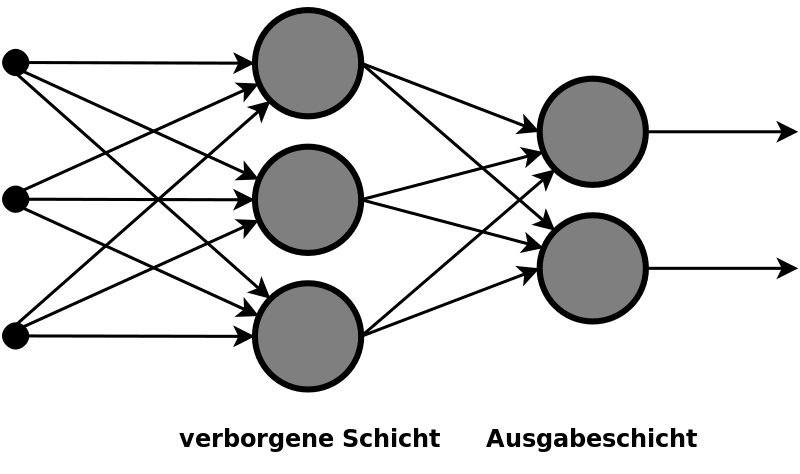
\includegraphics[totalheight=0.2\textheight]{Bilder/Multi-Layer_Neural_Network-Vector.png}
	\end{center}
	\caption{Zweischichtiges Netz (wiki)}
	\label{fig:Schichten}
\end{figure}
Ein jedes Neuron rechnet die hineinkommenden Eingabewerte mit einer zur Übertragungskante zugehörigen Gewichtung mit einer Übertragungsfunktion zusammen, die Anzahl der Eingaben ist hierbei unbegrenzt ("unlimited fan-in property" \cite{Rojas:1996:NNS:235222}). Die Übertragungsfunktion kann hierbei schlicht die Summe aller gewichteten Eingaben sein. Der errechnete Wert wird als Netzeingabe an die Aktivierungsfunktion gegeben. 
\\
\begin{figure}[h]
	\begin{center}
		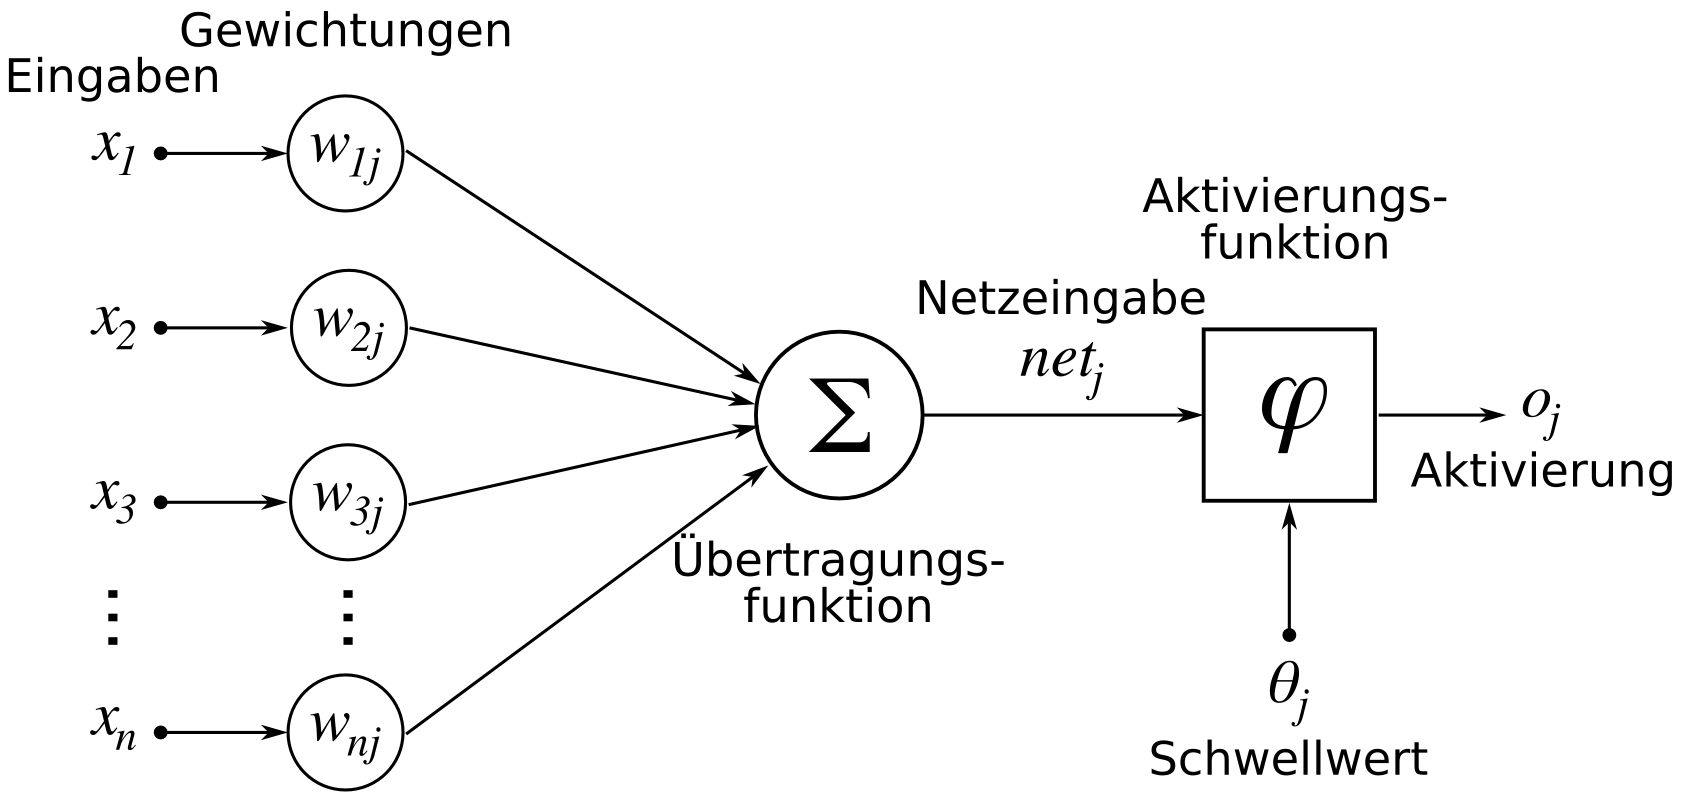
\includegraphics[totalheight=0.2\textheight]{Bilder/ArtificialNeuronModel_deutsch.png}
	\end{center}
	\caption{Schema eines künstlichen Neurons (wiki)}
	\label{fig:Neuron}
\end{figure} \\

Die Aktivierungsfunktion berechnet eventuell mit einem Schwellwert die Aktivierung des Neurons, welche dann an alle verbundenen Neuronen der nächsten Schicht gegeben wird. Die Aktivierungsfunktion kann beispielsweise eine simple Stufenfunktion sein, die allen Netzeingbaben kleiner des Schwellwertes eine Null und allen Eingaben größer gleich des Schwellwertes eine Eins zuweist.\\
Ein Neuron mit der gewichteten Summe aller Eingaben als Übertragungsfunktion und einer Stufenfunktion mit Schwellwert als Aktivierungsfunktion wird von Rojas Perzeptron bezeichnet \cite{Rojas:1996:NNS:235222} (Seite 60).
Ein feedforward-Netzwerk aus Perzeptrons, in dem jedes Neuron mit allen Neuronen der folgenden Schicht verbunden ist, wird als multilayer perceptron (kurz MLP) bezeichnet.
Ein neuronales Netz lernt die Abbildung zwischen den vorgegebenen Paaren von Eingabe- und Ausgabedaten durch Anpassung der Gewichte an den Kanten, nachdem es mit zufällig initialisierten Kantengewichten gestartet ist. Diese Anpassung geschieht beim MLP durch Fehlerrückführung (engl. backpropagation). Dabei wird der mittlere quadratische Fehler der berechneten Ausgabe gegenüber der vorgegebenen Ausgabe ermittelt und daraufhin unter Rücksichtnahme auf eine Lernrate mit Hilfe des Gradientenverfahren minimiert.
Vor der Anwendung eines künstlichen neuronalen Netzes für ein Problem stellt sich die Frage, ob dieses für das Problem geeignet ist. Dazu gibt es einige interessante mathematische Beweise.
Ein einzelnes Perzeptron kann alle linear separierbaren logischen Funktionen exakt approximieren \cite{Rojas:1996:NNS:235222} (Seite 62-63). 
Wobei lineare Separierbarkeit definiert ist als: Zwei Mengen von Pukten A und B .. (auf deutsch? ) \\

\begin{figure}[h]
	\begin{center}
		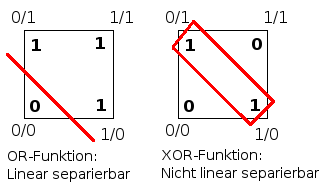
\includegraphics[totalheight=0.2\textheight]{Bilder/Lineare_Separierbarkeit.png}
	\end{center}
	\caption{Lineare Separierbarkeit von Funktionen (wiki)}
	\label{fig:Neuron}
\end{figure} 

Diese Beschränkung gilt allerdings nicht für ein Netzwerk von Neuronen. Bereits ein zweilagiges Netzwerk aus noch simpleren McCulloch-Pitts-Zellen kann jede beliebige logische Funktion berechnen \cite{Rojas:1996:NNS:235222} (Seite 37).
Für MLPs hat Cybenko \cite{cybenko:mcss} bewiesen, dass sie belieblige kontinuierliche Funktionen auf einer kompakten Teilmenge des euklidischen Raums $\mathbb{R}^n$ approximieren kann. Der entsprechende Satz hierzu ist das "universal approximation theorem".

\bigskip
\paragraph{Zusammenfassung:}
\textit{2-5 Sätze, BLA In diesem Kapitel hab ich gesehen BLA und jetzt sehen wir Z. Wie hängen die Sections dieses Kapitels zusammen und warum brachte es was das zu lesen.}


\chapter{Verwandte Arbeiten}
\textit{%
	Um weniger Umschreiben zu müssen führe ich zunächst zwei Kategorien von Lösungsansätzen ein. Danach erwähne ich kurz einige Arbeiten, dessen Themen sich mit dem dieser Arbeit überschneiden, und danach gehe ich noch etwas detailierter auf Veröffentlichungen mit hoher Ähnlichkeit und Relevanz ein.  
	Mini-Gliederung was jetzt kommt. Einleitung ist OPTIONAL!!!!
	In Sektion X steht, in Y steht.
}
\bigskip

\section{Leistungsvorhersage von Ein-/Ausgabe}


\section{Leistungsvorhersage mit Maschinellem Lernen}
Artificial neural networks for modelling and control of non-linear systems
\url{https://books.google.de/books?hl=de&lr=&id=tmTTBwAAQBAJ&oi=fnd&pg=PR9&dq=%22neural+networks%22+storage&ots=KyYA14xY1w&sig=yAQG0zn41xAHccDNaUWYd3L_ywI}


\section{Neuronale Netzen im Hochleistungsrechnen}

Viele Projekte verwenden Neuronale Netze für die Modellierung vom Gehirn....
http://world-comp.org/p2012/PDP3003.pdf

Machine Learning for Machines: Data-Driven Performance Tuning at Runtime Using Sparse Coding
SJ Tarsa - 2015 - dash.harvard.edu
... 83 5.2 Workload Models and Data Collection . . . . . 85 5.3 Predicting Storage
Performance with CART . . . . . 87 5.3.1 Applying CART to Multi-Tenant Scenarios . . . . .
87 5.3.2 Variation-Tolerant CART Using Workload Labels . . . . . ... 

Predicting disk drive failure at a central processing facility using an evolving disk drive failure prediction algorithm

ABER sie werden nur unzureichend eingesetzt für I/O und deswegen braucht es die Arbeit.

10-20 andere literatur


\section{Kategorisierung (woanders hin?)}
	Das Problem, die Zugriffszeiten auf Festplatten vorherzusagen, kann im wesentlichen durch zwei verschiedene Ansätze gelöst werden.\\ Zum einen kann man versuchen ein Modell des Festplattensystems zu erstellen, indem Hardwaredetails, wie die Rotationsgeschwindigkeit der Platte, die Reaktionszeit und Geschwindkeit des Lesekopfs, sowie das Zusammenspiel der Komponenten, bekannt sind oder entsprechende Parameter werden durch gezielte Untersuchung approximiert. (\textbf{stimmt das? Referenz?}) Mit diesem möglichst exakten Modell können dann Zugriffe simuliert und so deren Aufwand vorhergesagt werden. \\ Der zweite Ansatz ist auch der dieser Arbeit, es wird von dem eigentlichen Festplattensystem abstrahiert und stattdessen ein mathematisches Modell gesucht, das aus gemessenen Leistungswerten von Festplattenzugriffen die Werte von neuen Zugriffen ableitet. Ich unterscheide daher im Folgenden zwischen dem Modellierungssansatz (in der Fachliteratur etwa als analytic device modeling und simulation modeling bezeichnet)
, bei dem versucht wird das Festplattensystem nachzubilden und dem Interpolationsansatz, bei dem ein numerisches Modell entwickelt wird. Da hier ohne Wissen über die inneren Zustände des Systems modelliert wird, wird dieser Ansatz auch black-box modeling bezeichnet. (Quelle? Fourier assisted ml)
	
\section{Modellierungssansatz gegenüber Regressionsansatz}
	Die Nachteile von Modellen mit Modellierungssansatz liegen insbesondere daran, dass sie aufwendig zu konfigurieren sind "In fact, one of us (Oldfield) spent several months configuring DiskSim to model an existing device" \cite{Crume:2013:FML:2538542.2538561} (S.1) und naturgemäß schnell veraltern, da sie jeweils an spezielle Hardware angepasst sind. Der Vorteil dagegen ist, dass sie bei korrekter Konfiguration sehr präzise sind, wie z.B. hier gezeigt \cite{Ruemmler94anintroduction}. \\
	Der Interpolationsansatz ist in der Anwendung einfacher und flexibler, da es sich automatisch an das System anpasst. Dafür erwartet man aufgrund der fehlenden analytischen Einsicht ins System eine etwas schlechtere Präzision. \\ Für die Anwendung im HPC-Bereich spielt der analytische Ansatz eine untergeordnete Rolle, da hier unterschiedliche Festplattensysteme zusammenarbeiten und stark mit der Netzwerkarchitektur verstrickt sind, sodass eine entsprechende Analyse des Systems zu aufwendig wird. "Furthermore, [...] building an accurate model or simulator using white box method cannot be a genereal solution in serving a variety of very different workloads" \cite{DBLP:conf/npc/ZhangLZJC10} (S.2, Zeile 20-24).

\section{xxx}
	Im HPC Bereich ist die Leistungsanalyse generell ein wichtiger Punkt, so wird beispielsweise das Scheduling-Algorithmen vom Dateisystem simuliert \cite{Liu_towardssimulation}, hier wird DiskSim \cite{Bucy08thedisksim} zur Vorhersage der Festplattenzugriffszeiten genutzt, dabei nutzt DiskSim einen Modellierungssansatz (analytical simulation). Eine weitere Arbeit, in der ein Modellierungsansatz genutzt wird stammt von Lebrecht et al. \cite{Lebrecht:2009:10.1109/QEST.2009.31}.\\ 
	Bei Arbeiten, in denen ein Interpolationsansatz genutzt wird, werden verschiedene Data-Mining bzw. stochastischen Methoden angewandt, beispielsweise eine Kombination aus regression trees und support vector mashines  \cite{Dai:2012:SDP:2477169.2477214}, bagging classification und regression trees \cite{DBLP:conf/npc/ZhangLZJC10}. Verschiedene statistische Methoden werden von Kelly et al. untersucht \cite{Kelly04inducingmodels}.

\section{Fourier-Assisted Machine Learning}
Adam Crume et al. \cite{Crume:2013:FML:2538542.2538561} gehen davon aus, dass der entscheidende Faktor bei der Vorhersage von Zugriffszeiten in der Erkennung von periodischen Mustern liegt. Diese Annahme ist für eine einzelne Festplatte gerechtfertigt, da man die Zugriffstzeit grob in zwei Teile aufteilen kann, zum einen die Bewegung des Lesekopfs auf die richtige Spur und die Bewegung des Kopfes entlang der Spur zum richtigen Punkt, auch wenn diese beiden Bewegungen in der Realität überlappen. Jede Festplattenspur hat entsprechend des Radius eine andere Periodendauer.\\
Durch eine Fourier Analyse finden sie die Hauptfrequenzen heraus und können diese dann nutzen, um mit einem neuronalen Netz Vorhersagen zu treffen.
Eine Schwierigkeit in dieser Arbeit ist unter anderem, dass durch die große Anzahl Perioden nur ein kleiner Ausschnitt der Festplatte in seiner Gesamtheit, also alle möglichen Paare von Ausgangs- und Endspuren, untersucht werden kann. Die Priorität solcher Frequenzen für die exakte Leistungsvorhersage, ist im komplexen HPC-E/A-System zunächst einmal nicht zu erwarten, müsste allerdings untersucht werden.

\section{Predicting Performance of Non-Contiguos I/O with Machine Learning}
Direkt aus dem Bereich des Hochleistungsrechnens stammt die Arbeit von Kunkel et. al \cite{UMLTPTPONI15}. Hier wird versucht mit Hilfe von decision trees die performantesten Parameter für nicht zusammenhängende Zugriffe auf Dateien durch ROMIO, einer Implementierung von MPI-2 I/O, zu finden. Dabei sagen sie mit den decision trees die Performance für die verschiedenen Parameter auf den Daten voraus, sodass sie anhand dieser Vorhersagen die besten Parameter finden. (\textbf{habe ich das richtig verstanden}?) Mit dieser Methode haben sie es geschafft zufriedenstellende Ergebnisse zu erzielen. Die Simplizität von decision trees, beispielsweise können diese nur Entscheidungen als eine Aneinanderreihung von linearen Separationen des Werteraums treffen, lässt vermuten, dass mit Hilfe von komplexeren Data Mining - Methoden, wie neuronalen Netzen noch bessere Ergebnisse erzielt werden könnten. Hier findet sich ein potenzielles Anwendungsgebiet der Ergebnisse dieser Bachelorarbeit.

\paragraph{Zusammenfassung:}
\textit{2-5 Sätze, BLA In diesem Kapitel hab ich gesehen BLA und jetzt sehen wir Z. Wie hängen die Sections dieses Kapitels zusammen und warum brachte es was das zu lesen.}


\chapter{Gestaltung der Analyse}
\textit{%
	test
}
\bigskip

\section{Modell der Ein-/Ausgabe}
Zeit zum Bewegen des Lesekopfes + Zeit zum rotieren + lese-/schreibzeit + Aufrufprozedur mit festem Beitrag; t = tNetwork + tHDD +tMem \\
mit tHDD(deltaOffset, sizeInBlocks) = tBus(size) + f(deltaOffset)\\
track-to-track-seek-time, rotational time
Welche Abhängigkeiten gibt es, oder könnte es geben? Z.B. Umso größer die Size, desto länger die Lese-/Schreibzeit, umso größer Offset, desto größer die Seekzeit

\section{Leistungs- und Ausreißervorhersage}
Die Beiden Dinge, die ich versuche vorherzusagen. Warum? Unterschiede. 
\textbf{Macht es Sinn zu versuchen Ausreißer vorherzusagen?}

\section{Attribut Selektion und Generierung}
Korrelationen untersuchen, neues Attribute generieren (wesentlich für die verschiedenen Modelle)

\section{Modellklassen}
Zeitreihenanalyse, Aggregierung, Hybride

\section{Leistungsmetriken}
Welche Leistungsmerkmale werden warum untersucht?

\paragraph{Zusammenfassung:}
\textit{2-5 Sätze, BLA In diesem Kapitel hab ich gesehen BLA und jetzt sehen wir Z. Wie hängen die Sections dieses Kapitels zusammen und warum brachte es was das zu lesen.}


\chapter{Implementierung}
\textit{%
	test
}
\bigskip

\section{Untersuchte Modelle}
jeweils Beschreiben, wie die Daten hierfür vorbereitet werden mussten, was die Idee davon ist ( warum macht es Sinn, dies zu testen), (wie soll die Performance hier untersucht werden?, Design?)

\section{Bagging zur Leistungssteigerung}
Konzept und Anwendung

\section{Anwendung? und Parameter}
Wie wird mit Ausreißern umgegangen, wie werden sie definiert, Cross-Validation, Anzahl berechneter Netze pro Modell, threshold, Größe der Netze, lern- und fehler-funktionen,

\section{Verwendete Programmiersprache und Bibliotheken}

\section{Testsystem, Mistral}
Speziell die Hardware von Mistral, von hier kommen die Benchmarks
Zur Evaluation verschieben: Testsystem

\paragraph{Zusammenfassung:}
\textit{2-5 Sätze, BLA In diesem Kapitel hab ich gesehen BLA und jetzt sehen wir Z. Wie hängen die Sections dieses Kapitels zusammen und warum brachte es was das zu lesen.}


\chapter{Evaluierung}
\textit{%
	test
}
\bigskip
\section{Leistungsvorhersage}
Zu jedem Modell schreiben, welche Attribute und Parameter sich als geeignet herausgestellt haben. Ergebnisse anhand von Graphen veranschaulichen.\\
Ergebnisse für verschiedene Fälle vergleichen, seq,rnd,mistral vs pc?\\
Jeweils schreiben, ob bagging etwas bringt.
\subsection{Aggregationsmodelle}
\subsection{Zeitreihenmodelle}
\subsection{Hybridemodelle}

\section{Ausreißervorhersage}
\subsection{Aggregationsmodelle}
\subsection{Zeitreihenmodelle}
\subsection{Hybridemodelle}

\paragraph{Zusammenfassung:}
\textit{2-5 Sätze, BLA In diesem Kapitel hab ich gesehen BLA und jetzt sehen wir Z. Wie hängen die Sections dieses Kapitels zusammen und warum brachte es was das zu lesen.}

\chapter{Fazit}
\label{Fazit}
Welche Modelle sind für welchen Fall erfolgsversprechend?
Eignen sich Neuronale Netze zum Vorhersagen von E/A-Leistung im HPC?\\
Wo könnten die Ergebnisse eingesetzt werden?\\
Was müsste als nächstes getan werden?\\

\bibliographystyle{alpha}
\bibliography{literatur}

\listoffigures

\listoftables

\lstlistoflistings

\begin{appendices}

\chapter{Anhangskapitel}

Lorem ipsum dolor sit amet, consetetur sadipscing elitr, sed diam nonumy eirmod tempor invidunt ut labore et dolore magna aliquyam erat, sed diam voluptua.
At vero eos et accusam et justo duo dolores et ea rebum.
Stet clita kasd gubergren, no sea takimata sanctus est Lorem ipsum dolor sit amet.

\end{appendices}

\newpage

\thispagestyle{empty}

\chapter*{}

\section*{Erklärung}

Ich versichere, dass ich die Arbeit selbstständig verfasst und keine anderen, als die angegebenen Hilfsmittel -- insbesondere keine im Quellenverzeichnis nicht benannten Internetquellen -- benutzt habe, die Arbeit vorher nicht in einem anderen Prüfungsverfahren eingereicht habe und die eingereichte schriftliche Fassung der auf dem elektronischen Speichermedium entspricht.

\smallskip

\textbf{Optional:} Ich bin mit der Einstellung der Bachelor-Arbeit in den Bestand der Bibliothek des Fachbereichs Informatik einverstanden.

\bigskip
\bigskip
\bigskip

Hamburg, den 01.01.2012  \quad \dotfill

\end{document}
